%   % !TEX root = ../../VIII,3_Rahmen-TeX_8-1.tex
%
%
%   Band VIII, 3 N.~??A41
%   Signatur/Tex-Datei: LH_35_09_16_008
%   RK-Nr. 41174
%   Überschrift: Paradoxon circa firmitatem
%   Modul: Mechanik / Festigkeit
%   Datierung: [Ende Januar 1683 bis Mitte 1685 (?)]
%   WZ: (keins), aber vielleicht Papier mit Karos
%   SZ: (keins)
%   Bilddateien (PDF): LH_35_09_16_008v_d (insgesamt: eine)
%
%
\selectlanguage{ngerman}%
\frenchspacing%
%
\begin{ledgroupsized}[r]{120mm}%
\footnotesize%
\pstart%
\noindent%
\textbf{Überlieferung:}%
\pend%
\end{ledgroupsized}%
\begin{ledgroupsized}[r]{114mm}%
\footnotesize%
\pstart%
\parindent -6mm%
\makebox[6mm][l]{\textit{L}}%
Notiz:
LH~XXXV~9,~16 Bl.~8.
Ein Zettel (8,5 x 5,5 cm).
Text auf Bl.~8~v\textsuperscript{o}.
Auf Bl.~8~r\textsuperscript{o} % stehen die 
finden sich nur die Zeilenanfänge eines durch Beschnitt verlorenen Textes
(das Fragment wird angesichts des Überlieferungszustandes diplomatisch wiedergegeben): % (die Streichung darin wird diplomatisch wiedergegeben, da die fragmentarische Überlieferung keine genauere Aussage über ihren Status zulässt):
% \newline
\textit{Es wu}$\langle\dots\rangle$
\lbrack/\rbrack\ \textit{ersuchs}\textlangle\dots\textrangle\
\lbrack/\rbrack\ \textit{Künste} \textlangle\dots\textrangle\
\lbrack/\rbrack\ \textit{\sout{Osterod}}\textlangle\dots\textrangle\
\lbrack/\rbrack\ \textit{noch geri}\textlangle\dots\textrangle\
\lbrack/\rbrack\ \textit{werden} \textlangle\dots\textrangle\
\pend%
\end{ledgroupsized}%
%
%
%\normalsize
\vspace*{5mm}%
\begin{ledgroup}%
\footnotesize%
\pstart%
\noindent%
\textbf{Datierungsgründe:}
Das samt der vorliegenden Notiz N.~20 überlieferte Textfragment ist wahrscheinlich auf Leibnizens Pläne bezogen, Windkünste für den Harzbergbau einzurichten.\protect\index{Ortsregister}{Harz}
Hiermit beschäftigte er sich hauptsächlich in den Jahren 1680 bis 1686 (siehe \textit{LSB} I, Supplementband Harzbergbau 1692\textendash1696, Einleitung, S.~XXIX\textendash XXXI\cite{01337}).
Die Notiz N.~20 sollte daher innerhalb dieser Zeitspanne verfasst worden sein.
Die vermutliche Entstehungszeit lässt sich jedoch weiter eingrenzen, indem man die inhaltliche Verwandtschaft beachtet, die zwischen N.~20 und anderen in diesem Band edierten Texten besteht, deren thematischer Schwerpunkt die Reißfestigkeit gespannter Saiten oder Seile ist.
An erster Stelle ist die im Zeitraum von Ende Januar 1683 bis Ende des Jahres 1684 verfasste Aufzeichnung N.~17 zu erwähnen, die hauptsächlich auf die Frage eingeht, unter welcher Spannkraft Saiten oder Seile reißen.
Auch mit der eigenhändig auf den 29.~April (9.~Mai) 1685 datierten Aufzeichnung N.~26 weist N.~20 eine starke inhaltliche Verwandtschaft auf, da N.~26 in ähnlicher Weise mit den Bedingungen befasst ist, unter denen gespannte Seile reißen.
Die Annahme liegt daher nahe, dass auch N.~20 in der Zeitspanne zwischen Ende Januar 1683 und Mitte 1685 verfasst worden sein dürfte.
Dieser Datierungsvorschlag wird ferner dadurch bestätigt, dass seit dem Spätsommer 1682 Leibniz sich ohnehin mit E.~Mariotte\protect\index{Namensregister}{\textso{Mariotte}, Edme, Seigneur de Chazeuil ca. 1620\textendash1684} über Fragen der Festigkeit und Elastizität austauschte, woraus der umfangreiche Textkomplex N.~14 entstand (siehe die editorische Vorbemerkung hierzu, S.~\pageref{AE_1684_319-325_intro_jecg}\,ff.).
Und die Beschäftigung mit Themen der Akustik, wie sie im Textkomplex N.~12 belegt ist, war Leibniz noch in der ersten Hälfte 1685 ein Grund dafür, Überlegungen über das Verhalten elastischer Körper wie Saiten anzustellen (siehe zur Entstehung von N.~12 die editorische Vorbemerkung, S.~\pageref{cogitationesnovae-intro}\,ff.).
Eine frühere (ab 1680) oder spätere Datierung der Notiz N.~20 lässt sich jedoch nicht ausschließen.
Für eine spätere Entstehungszeit kämen vor allem die Jahre 1693 bis 1696 in Frage, als Leibniz seine zweiten bergwerktechnischen Versuche im Harz unternahm.
% \pend%
% \pstart%
\pend%
\end{ledgroup}%
%
%
\selectlanguage{latin}%
\frenchspacing%
%
%\newpage%
 \vspace{8mm}
%
\count\Bfootins=1000
\count\Afootins=1000
\count\Cfootins=1000
%
%
\pstart
\noindent
\lbrack8~v\textsuperscript{o}\rbrack\
Interdum fit ut debilitemus
quod fortificare volumus,
quia interdum fortificato toto,
eo ipso
(\protect\vphantom)%
quod mirum est%
\protect\vphantom()
debilitatur pars.
Cujus paradoxi\protect\index{Sachverzeichnis}{paradoxon}
haec est ratio,\protect\index{Sachverzeichnis}{ratio paradoxi}
quod ea
quae ubique aeque firma sunt
non franguntur facile,
at si unam partem fortiorem reddideris
%
% \edtext{}{%
% \lemma{fortiorem}\Bfootnote{%
% \textit{(1)}~reddideris \textit{(2)}~reddideris~\textit{L}}}
%
facilius continget fractio.\protect\index{Sachverzeichnis}{fractio}
Ut\edlabel{LH_35_09_16_008v_gleichSpann_shqe-1}
%
\edtext{si sit filum\protect\index{Sachverzeichnis}{filum} \textit{ABC}
unco\protect\index{Sachverzeichnis}{uncus} in \textit{A} suspensum
et a pondere \textit{C} tensum,\protect\index{Sachverzeichnis}{pondus tendens}
id patet tendi ubique,
sed si portio \textit{AB}}{%
\lemma{si}\Bfootnote{%
\textit{(1)}~\textit{AB} portio fili unco in \textit{A} suspensi
\textit{(2)}~sit filum \lbrack...\rbrack\ portio \textit{AB}
~\textit{L}}}
%
sit fortior
quam ut tendi possit,
portio \textit{BC},
quae sola vim tensionis\protect\index{Sachverzeichnis}{vis tensionis} totam ferre cogitur, rumpetur.%
\edlabel{LH_35_09_16_008v_gleichSpann_shqe-2}
Unde patet tales observationes\protect\index{Sachverzeichnis}{observatio}
quae vulgo praxi\protect\index{Sachverzeichnis}{praxis} ascribuntur,
a vera theoria\protect\index{Sachverzeichnis}{theoria} pendere.
\pend%
\newpage
%
%
%  \newpage% 
  \vspace{1.5em}%	% Diagramm Fig.~1
  \centerline{\hspace*{-16mm}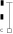
\includegraphics[width=0.09\textwidth]{gesamttex/edit_VIII,3/images/LH_35_09_16_008v_d.pdf}}%
  \vspace*{-5.0em}
  \centerline{\hspace*{16mm}\lbrack\textit{Fig.~1}\rbrack}%
  \label{LH_35_09_16_008v_Fig.1}%
  \count\Bfootins=1200
\count\Afootins=1200
\count\Cfootins=1200
%  \vspace{2em}%
%  \newpage%
%
%
%    %    %    %    Ende des Textes auf Bl. 8v